\documentclass[../main.tex]{subfiles}
\begin{document}
\chapter{Resultados}
Para conseguir resultados significativos, no sólo debieron seguirse los métodos descritos en el capítulo anterior, sino que también estos se realizaron en un orden particular, que permitió determinar las condiciones de las técnicas subsecuentes además de prevenir mediciones innecesarias. En la figura \ref{fig:resdiag} se puede observar un diagrama del orden seguido.
\begin{figure}[H]
    \centering
    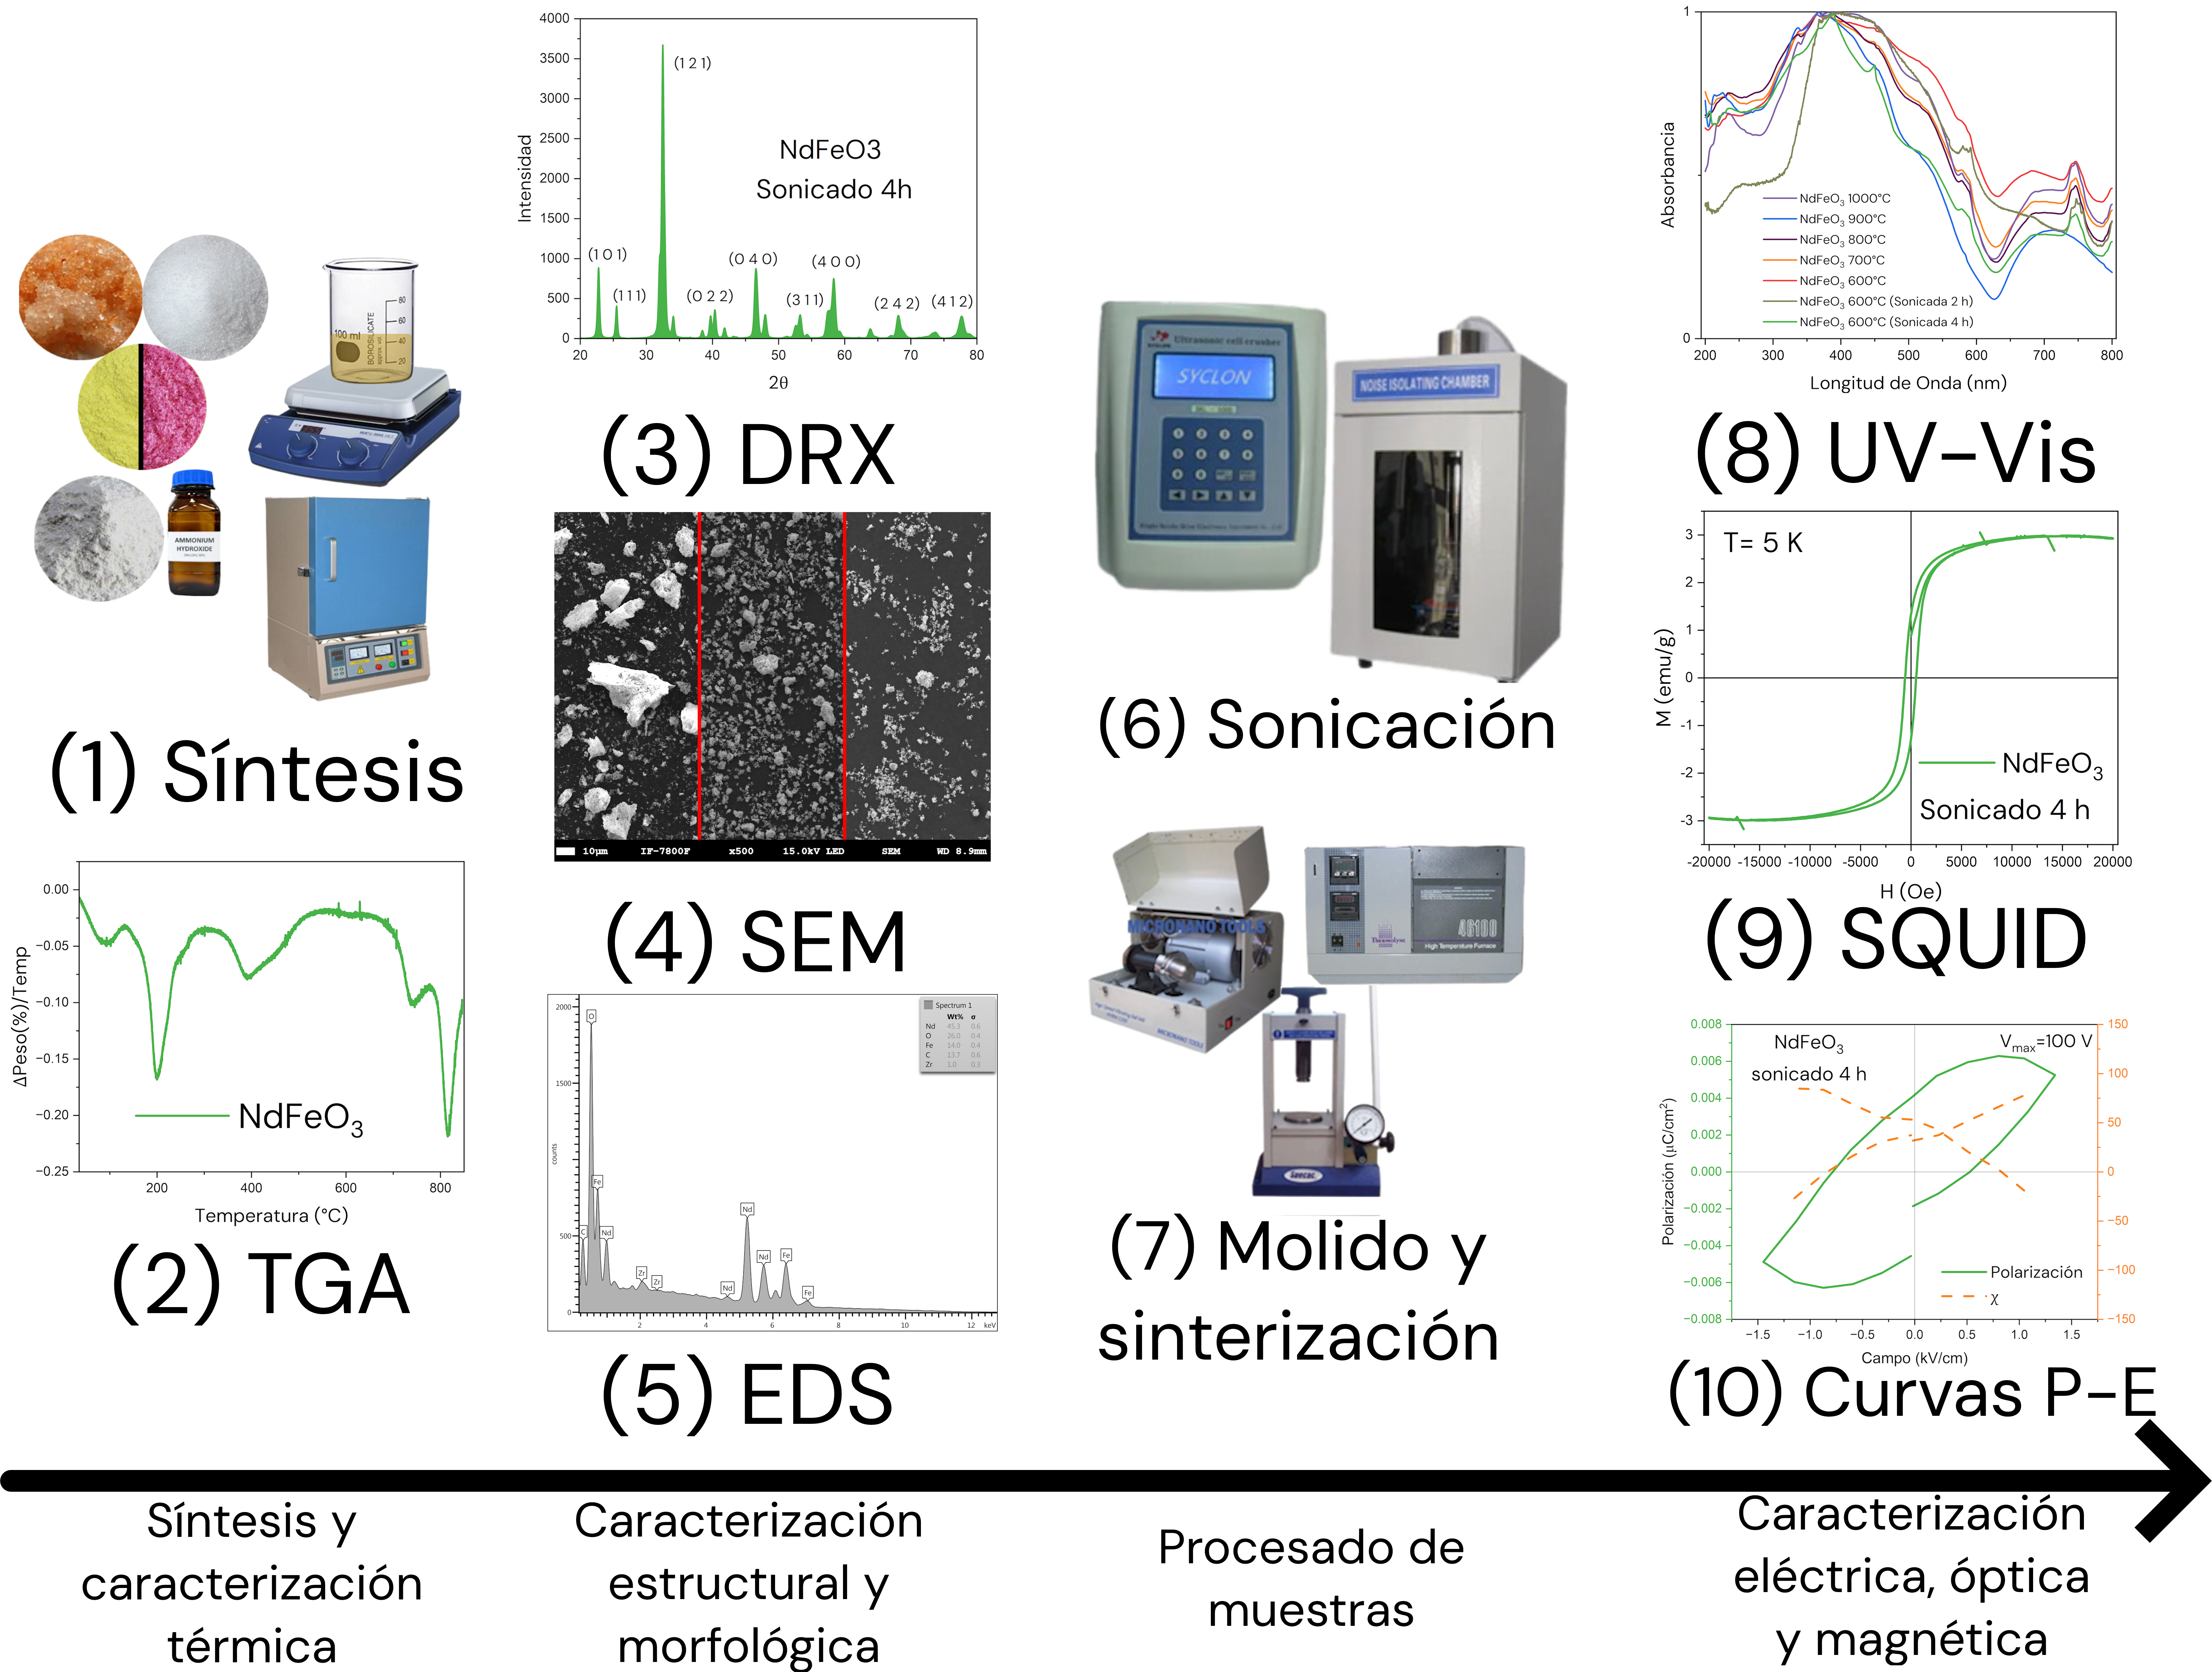
\includegraphics[width=0.7\textwidth]{fig/diagresultados.png}
    \caption{Resultados obtenidos mediante las técnicas de síntesis y caracterización descritas en el capítulo 4.}
    \label{fig:resdiag}
\end{figure}
\section{Muestras Sintetizadas} \label{sec:sintesis}
Se sintetizaron un total de 8 muestras de 1g de cada ortoferrita. Una muestra de cada una fue reservada para realizar un análisis termogravimétrico. A través de éste, se determinó la temperatura mínima de calcinación para ambas ortoferritas, como se reporta en la sección \ref{sec:TGA}.

Con estas temperaturas en mente, 600\gradoC{} para el \neod{} y 700\gradoC{} para el \sama{}, se calcinaron el resto de muestras, 4 muestras de \neod{} se calcinaron a 600\gradoC{}, para las otras 3 se aumentó la temperatura 100\gradoC{} por cada una, es decir, se calcinaron a 700, 800 y 900\gradoC{} respectivamente.

Por otro lado, para el \sama{} se calcinaron 4 muestras a 700\gradoC{}, aumentando la temperatura de la misma forma que en el caso del \neod{} para las otras 3, es decir, se calcinaron a 800, 900 y 1000\gradoC{} respectivamente.
\section{Caracterización}
\subsection{Análisis Térmico} \label{sec:analisistermico}
\subsubsection{Análisis Termogravimétrico} \label{sec:TGA}
Se realizó un análisis termogravimétrico a ambas ortoferritas, lo cual dió como resultado las siguientes curvas de masa contra temperatura:
\begin{figure}[H]
    \centering
    \includegraphics[width=0.4\textwidth]{fig/TGA-NdFeO3.png}
    \quad
    \includegraphics[width=0.4\textwidth]{fig/TGA-SmFeO3.png}
    \caption{Análisis termogravimétrico de las ortoferritas.}
    \label{fig:TGAres}
\end{figure}
Se obtuvo la derivada de la masa respecto a la temperatura:
\begin{figure}[H]
    \centering
    \includegraphics[width=0.4\textwidth]{fig/TGA-derNdFeO3.png}
    \quad
    \includegraphics[width=0.4\textwidth]{fig/TGA-derSmFeO3.png}
    \caption{Derivada de la masa respecto a la temperatura para ambas ferritas.}
    \label{fig:derTGAres}
\end{figure}
Se pueden observar 3 regiones distintas donde ocurren cambios térmicos en la muestra:
\begin{table}[H]
    \centering
    \begin{tabular}{|c|c|}
        \hline
        Zona & Temperatura\\
        & aproximada\\\hline\hline
        1&100-200\gradoC{}\\
        \hline
        2&300-500\gradoC\\\hline
        3&>700\gradoC\\
        \hline
    \end{tabular}
    \caption{Regiones donde cambia el comportamiento de la masa respecto a la temperatura para ambas muestras.}
    \label{tabla:TGAtabla}
\end{table}
La región 1 coincide con las temperaturas a la que el agua se evapora y se combustiona la fase orgánica en la muestra. Se piensa que la formación de la fase cristalina ocurre en las regiones 2 y 3.
\subsection{Análisis Estructural, Morfológico y de Composición} \label{sec:analisisestruc}

\subsubsection{Microscopía Electrónica de Barrido}
Se estudió la morfología de las partículas sintetizadas a través de esta técnica, dando como resultado imágenes como las que se muestran en la figura \ref{fig:resSEMsonic}.

En general, se observa que estas partículas presentan una estructura porosa, la cual se rompe después de ser sometida a un proceso de sonicación, siendo esto evidente al comparar las figuras \ref{fig:resSEMsonic} (a) y \ref{fig:resSEMsonic} (b), las cuales muestras a las ortoferritas de \neod{} calcinada a 600\gradoC{} y \sama{} calcinada a 700\gradoC{} respectivamente, con las figuras \ref{fig:resSEMsonic} (c) y\ref{fig:resSEMsonic}(d), en donde se muestran éstas mismas muestras después de ser sonicadas por 2 horas a 292W, además de las figuras \ref{fig:resSEMsonic} (e) y \ref{fig:resSEMsonic} (f), donde éstas muestras fueron sonicadas por 4 horas a la misma potencia.
\begin{figure}[H]
    \centering
    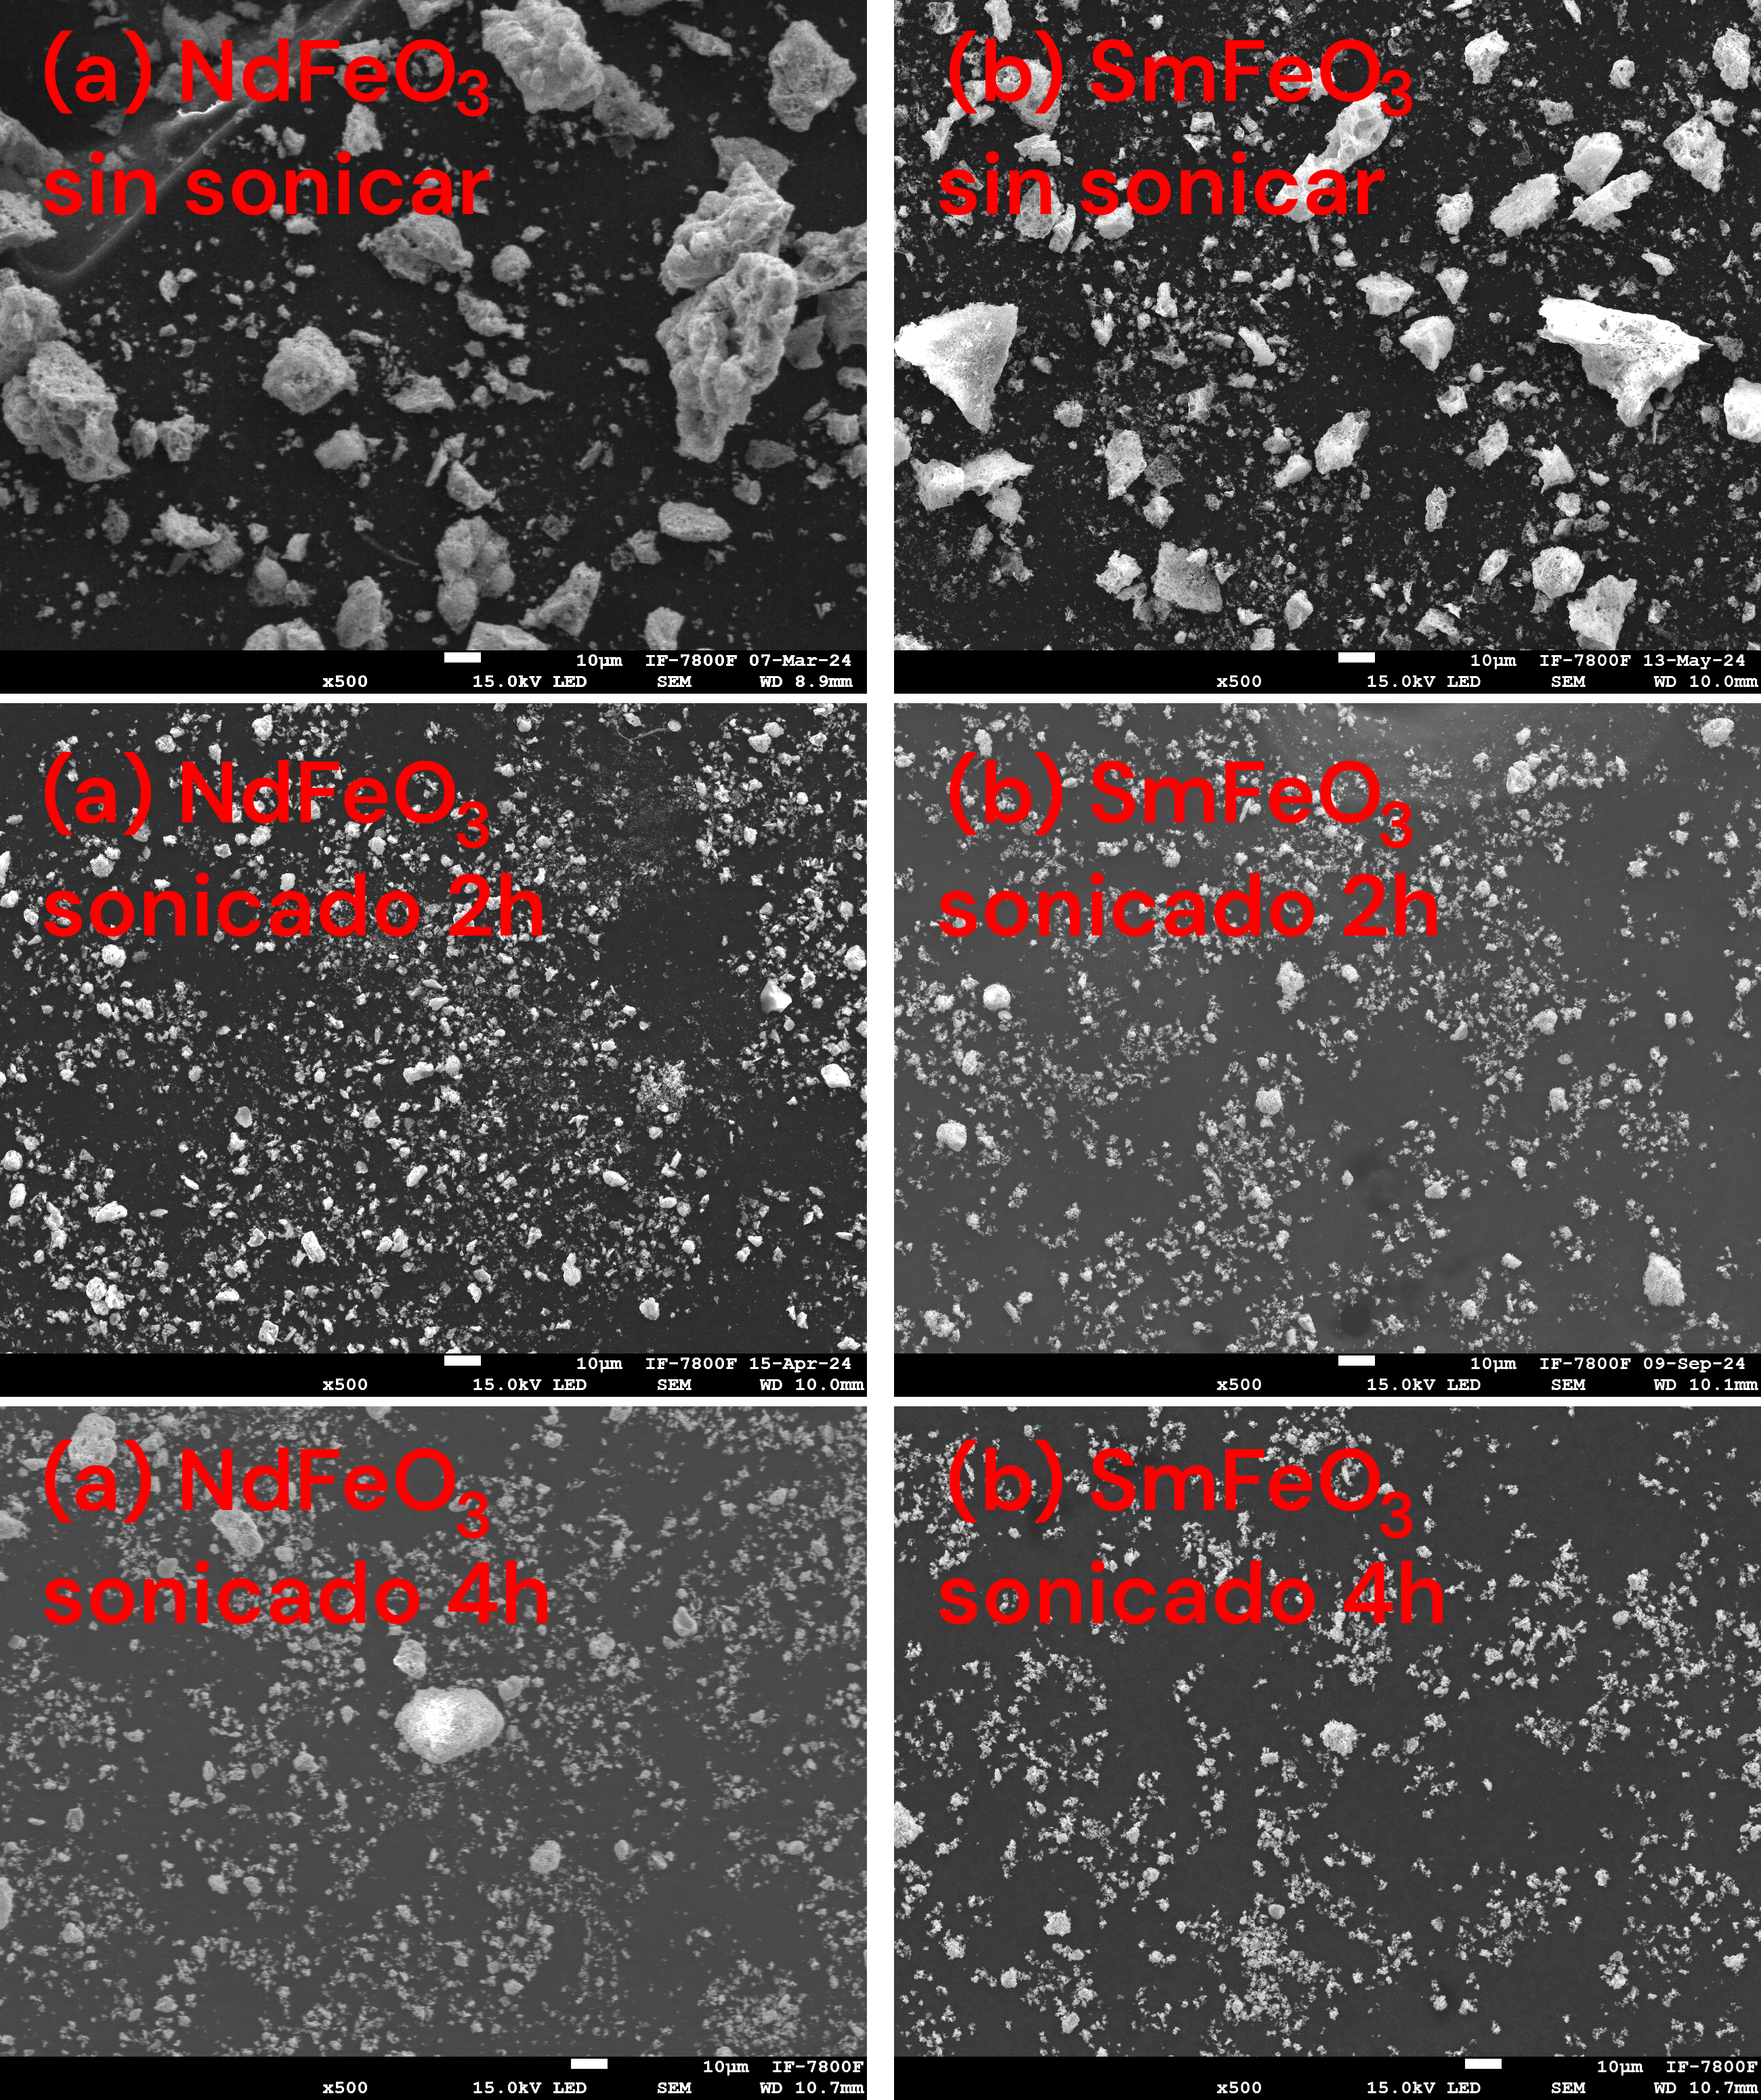
\includegraphics[width=0.7\textwidth]{fig/ressem.png}
    \caption{Imágenes obtenidas a través de SEM. Amplificación x500.}
    \label{fig:resSEMsonic}
\end{figure}
Como ya se describió en la sección \ref{sec:analisisestadistico}, los tamaños de partícula fueron obtenidos haciendo uso de \textit{ImageJ}.

El primer método descrito en esa sección dió como resultado los siguientes diámetros de partícula promedio:
\begin{table}[H]
    \centering
    \begin{tabular}{|c||c|c|}
        \hline
        Muestra & Temperatura de & Diámetro \\
        & calcinación & promedio \\
        \hline
        \hline
        \multirow{6}{*}{\rotatebox[origin=c]{90}{\neod{}}} & 600\gradoC{} & 1.49 $\pm$ 0.028 \\
        \cline{2-3}
        & 600\gradoC{}, sonicada 2 h & 1.00 $\pm$ 0.035 \\
        \cline{2-3}
        & 600\gradoC{}, sonicada 4 h & 0.98 $\pm$ 0.023 \\
        \cline{2-3}
        & 700\gradoC{} & 1.76 $\pm$ 0.047 \\
        \cline{2-3}
        & 800\gradoC{} & 2.5 $\pm$ 0.087 \\
        \cline{2-3}
        & 900\gradoC{} & 2.66 $\pm$ 0.065 \\
        \hline
        \hline
        \multirow{6}{*}{\rotatebox[origin=c]{90}{\sama{}}} & 700\gradoC{} & 2.01 $\pm$ 0.051 \\
        \cline{2-3}
        & 700\gradoC{}, sonicada 2 h & 1.81 $\pm$ 0.037 \\
        \cline{2-3}
        & 700\gradoC{}, sonicada 4 h & 1.66 $\pm$ 0.045 \\
        \cline{2-3}
        & 800\gradoC{} & 1.91 $\pm$ 0.034 \\
        \cline{2-3}
        & 900\gradoC{} & 1.97 $\pm$ 0.029 \\
        \cline{2-3}
        & 1000\gradoC{} & 2.02 $\pm$ 0.055 \\
        \hline
        \end{tabular} 
    \caption{Tamaño promedio de partícula según la temperatura de calcinación para ambas ferritas.}
    \label{tabla:restamañoprom}
\end{table}
\begin{figure}[H]
    \centering
    \includegraphics[width=0.9\textwidth]{fig/restamañoprom.png}
    \caption{Gráfica del tamaño promedio de partícula según la temperatura de calcinación.}
    \label{fig:restamañoprom}
\end{figure}

Por otro lado, el segundo método descrito en la sección \ref{sec:analisisestadistico} dió como resultado los siguientes porcentajes:
\begin{table}[H]
    \centering
    \begin{tabular}{|c||c|c|}
        \hline
        Muestra & Temperatura de & Porcentaje \\
        & calcinación & $\leq1$ $\mu$m \\
        \hline
        \hline
        \multirow{6}{*}{\rotatebox[origin=c]{90}{\neod{}}} & 600\gradoC{} & 67.29 $\pm$ 4.0796 \\
        \cline{2-3}
        & 600\gradoC{}, sonicada 2 h & 80.87 $\pm$ 0.79942 \\
        \cline{2-3}
        & 600\gradoC{}, sonicada 4 h & 87.1 $\pm$ 1.29258 \\
        \cline{2-3}
        & 700\gradoC{} & 58.8 $\pm$ 1.84167 \\
        \cline{2-3}
        & 800\gradoC{} & 61.27 $\pm$ 1.80513 \\
        \cline{2-3}
        & 900\gradoC{} & 53.85 $\pm$ 2.55817 \\
        \hline
        \hline
        \multirow{6}{*}{\rotatebox[origin=c]{90}{\sama{}}} & 700\gradoC{} & 55.18 $\pm$ 2.1034 \\
        \cline{2-3}
        & 700\gradoC{}, sonicada 2 h & 88.13 $\pm$ 1.08097 \\
        \cline{2-3}
        & 700\gradoC{}, sonicada 4 h & 92.62 $\pm$ 0.91496 \\
        \cline{2-3}
        & 800\gradoC{} & 44.4 $\pm$ 2.5047 \\
        \cline{2-3}
        & 900\gradoC{} & 62.28 $\pm$ 2.49791 \\
        \cline{2-3}
        & 1000\gradoC{} & 44.46 $\pm$ 2.64018 \\
        \hline
\end{tabular} 
    \caption{Porcentaje de partículas con diámetro $\leq$1 $\mu$m según la temperatura de calcinación para ambas ferritas.}
    \label{tabla:resporcentaje}
\end{table}
\begin{figure}[H]
    \centering
    \includegraphics[width=0.9\textwidth]{fig/resporcentaje.png}
    \caption{Gráfica del porcentaje de partículas con diámetro $\leq$1 $\mu$m según la temperatura de calcinación.}
    \label{fig:resporcentaje}
\end{figure}
Estos datos sugieren una correlación entre la temperatura de calcinación y el diámetro promedio, en particular para el \neod{}.

Se observa que el tamaño de partícula decrece, al mismo tiempo que aumenta considerablemente el porcentaje de partículas de diámetro $\leq1$ $\mu$m. 

Sin embargo, duplicar el tiempo de sonicación no cambia los resultados de manera significativa, por lo cual se piensa que este proceso sólo rompe las partículas más grandes, pero no es lo suficientemente potente para fragmentar las más pequeñas.
\subsubsection{Espectroscopía de Dispersión de Energía}
Esta técnica reveló los elementos presentes en las muestras introducidas al microscopio electrónico de barrido, lo cual permite hallar posibles contaminantes, además de delimitar las posibles estructuras cristalinas a tomar en cuenta en el análisis de la difracción de rayos X de la sección \ref{sec:analisisDRX}.

En ninguna de las mediciones se encontraron contaminantes externos, a excepción de carbono, el cuál puede explicarse debido a que la cinta utilizada para la preparación de muestras está hecha de este material, esto se reporta en las tablas \ref{tab:EDSNd} y \ref{tab:EDSSm}.

\begin{table}[H]
    \begin{tabular}{|c||c|c|c|c|c|c|c|}
        \hline
        Elem. &600\gradoC{} Son.&600\gradoC{} Son.&600\gradoC{}&700\gradoC{}&800\gradoC{}&900\gradoC{}&1000\gradoC{}\\
        &2h wt\%&4h wt\%&wt\%&wt\%&wt\%&wt\%&wt\%\\
        \hline\hline
        Fe & 20.33$\pm$0.78 &$21.00\pm0.77$& 19.94$\pm$0.68 & 22.23$\pm$1.01 & 20.31$\pm$0.67 & 21.0$\pm$1.04 & 18.37$\pm$2.06 \\
        Nd & 47.88$\pm$0.92 &$58.44\pm0.87$& 50.45$\pm$0.85 & 58.93$\pm$1.21 & 56.47$\pm$0.83 & 44.7$\pm$1.18 & 78.72$\pm$2.12 \\
        O & 31.79$\pm$0.70 &$20.56\pm0.56$& 21.71$\pm$0.54 & 11.04$\pm$0.57 & 15.06$\pm$0.45 & 20.4$\pm$0.57 & 2.92$\pm$0.60 \\
        C & 0 & 0 & 7.91$\pm$0.64 & 7.8$\pm$0.82 & 8.16$\pm$0.56 & 13.4$\pm$0.67 &0 \\ 
        \hline
        \end{tabular} 
            \caption{EDS de las muestras de \neod{}.}
            \label{tab:EDSNd}
        \end{table}
        \begin{table}[H]
            \centering
        \begin{tabular}{|c||c|c|c|c|c|c|}
        \hline
        Elem. &700\gradoC{} Son.&700\gradoC{} Son.&700\gradoC{}&800\gradoC{}&900\gradoC{}&1000\gradoC{}\\
        &2h wt\%&4h wt\%&wt\%&wt\%&wt\%&wt\%\\
        \hline\hline
        Fe &$13.78\pm0.52$&$19.48\pm1.48$& 7.51$\pm$0.42 & 22.31$\pm$0.93 & 22.51$\pm$3.03 & 17.44$\pm$0.83 \\
        Sm &$38.42\pm0.74$&$48.22\pm1.95$& 21.84$\pm$0.69 & 61.28$\pm$1.03 & 63.03$\pm$3.57 & 57.71$\pm$1.82 \\
        O &$18.74\pm0.45$&$15.64\pm1.00$& 15.95$\pm$0.47 & 16.41$\pm$0.58 & 14.46$\pm$1.78 & 20.81$\pm$0.78 \\
        C &$29.16\pm0.62$&$16.66\pm1.53$& 0 & 54.68$\pm$0.77 & 0 & 4.13$\pm$2.17 \\ 
        \hline
        \end{tabular} 
            \caption{EDS de las muestras de \sama{}.}
            \label{tab:EDSSm}
\end{table}
\subsubsection{Difracción de Rayos X} \label{sec:analisisDRX}
\begin{figure}[H]
    \centering
    \includegraphics[width=0.7\textwidth]{fig/drxtemp.png}
    \caption{Gráfica Rietveld.}
    \label{fig:drxrietveld}
\end{figure}

\subsection{Análisis Óptico, Magnético y Eléctrico} \label{sec:analisisoptmagelec}
\subsubsection{Espectroscopía UV-Vis}

\subsubsection{Magnetometría VSM}

\paragraph{M vs T}

\paragraph{\textchi{} vs T}

\paragraph{M v H}
\subsubsection{Curvas P-E}
\end{document}